\documentclass[10pt,a4paper]{article}
\usepackage[utf8]{inputenc}
\usepackage[T1]{fontenc}
\usepackage[brazil]{babel}
\usepackage{geometry}
\usepackage{booktabs}
\usepackage{tabularx}
\usepackage{amsmath,amssymb}
\usepackage{graphicx}
\usepackage{hyperref}
\usepackage{microtype}
\usepackage{xcolor}
\usepackage{colortbl}
\usepackage{enumitem}
\usepackage{fancyhdr}
\usepackage{makecell}
\usepackage{siunitx}
\usepackage{icomma}

\geometry{left=18mm,right=18mm,top=22mm,bottom=22mm}
\pagestyle{fancy}
\fancyhf{}
\rhead{\footnotesize Pesquisa de Sistemas: SLMs sob Restrições Severas de VRAM}
\lhead{\footnotesize GPU Lab Homelab | Engenharia de Sistemas e Ciência de Dados}
\rfoot{\footnotesize Página \thepage}

\hypersetup{
    colorlinks=true,
    linkcolor=blue!70!black,
    citecolor=blue!70!black,
    urlcolor=blue!70!black
}

\newcolumntype{C}{>{\centering\arraybackslash}X}
\newcolumntype{L}[1]{>{\raggedright\arraybackslash}p{#1}}

\title{\textbf{\LARGE Avaliação Empírica, Comportamental e de Engenharia de Sistemas de Modelos de Linguagem sob Restrições Severas de VRAM}\\[0.4em]
\large Uma Investigação Experimental Controlada com Ciência de Dados em NVIDIA GeForce GTX 1050 Ti}
\author{\textbf{Anderson Tavares} \\ Laboratório de Inteligência Artificial e Engenharia de Infraestrutura \\ \url{https://github.com/AndersonTavares0/llm-research-bench}}
\date{24 de outubro de 2026}

\begin{document}

\maketitle

\begin{abstract}
A inferência local em dispositivos de borda utilizando Modelos de Linguagem Pequenos (SLMs, 2B--4B parâmetros) assegura soberania de dados e latência determinística para servidores privados e nós autônomos. Entretanto, operar sob restrições físicas de memória severas ($\le 4096$ MiB de VRAM) impõe compromissos rigorosos entre precisão de quantização, execução especulativa, largura de banda efetiva e alinhamento de segurança. Este artigo apresenta um estudo experimental controlado conduzido em uma GPU NVIDIA GeForce GTX 1050 Ti (4096 MiB GDDR5, barramento de 128 bits, $112\text{ GB/s}$ de largura de banda teórica, Compute Capability 6.1) em container Proxmox VE LXC dedicado (CT 108). Quatro modelos (\textbf{Gemma-4-E2B-it}, \textbf{Qwen-3.5-4B}, \textbf{Qwen-3.5-2B} e \textbf{Llama-3.2-3B}) foram avaliados sob o runtime \texttt{llama-server} (commit b4120+). A telemetria de hardware foi capturada continuamente via \texttt{libnvidia-ml.so.1} a cada 250\,ms. Uma ablação controlada de decodificação especulativa Multi-Token Prediction (MTP) com $N=15$ repetições isolou um ganho estatisticamente significante de \textbf{30,9\%} no throughput médio global ($42,21 \pm 5,99$ vs $32,25 \pm 3,23$ tok/s, IC 95\%, $t$ de Welch = 3,139, $p = 0,0024$, $d$ de Cohen = 1,146) e de \textbf{33,2\%} em regime estacionário aquecido ($44,95$ vs $33,75$ tok/s), mantendo alocação estável de 2038 MiB. A análise controlada de quantização do Gemma-4-E2B revelou que o formato IQ4\_XS entrega vantagem de 59,3\% em regime aquecido sobre o Q4\_K\_M ($41,92$ vs $26,34$ tok/s, $t = 27,20$, $p = 3,59 \times 10^{-9}$). Em segurança adversária, todos os modelos recusaram ataques diretos (100\% de recusa contra CVE-2021-44228, keyloggers em C++ e DAN), mas sucumbiram uniformemente à injeção indireta de prompt encapsulada em logs de sistema (0\% de resistência), evidenciando que o alinhamento pós-treinamento falha em segregar instruções operacionais de dados contextuais não confiáveis.
\end{abstract}

\vspace{0.6em}
\noindent\textbf{Palavras-chave:} Modelos de Linguagem Pequenos, Restrições Severas de VRAM, Modelo Roofline, Decodificação Especulativa, Telemetria NVML, Teste de Hipóteses, Injeção Indireta de Prompt.

\section{Introdução e Fundamentação Teórica de Sistemas}

A execução local de assistentes e agentes inteligentes no ambiente de borda e homelab requer inferência autônoma sem dependências de nuvem pública. Em placas gráficas dedicadas de entrada como a NVIDIA GeForce GTX 1050 Ti (4096 MiB GDDR5, 768 núcleos CUDA, $B_{\text{teor}} = 112,0\text{ GB/s}$, TDP de 75W), o barramento de memória constitui o principal gargalo físico durante a geração autorregressiva.

\subsection{Modelo Roofline para a Microarquitetura Pascal}
A eficiência de inferência é modelada pela intensidade aritmética operacional $I$, definida como a razão entre operações de ponto flutuante executadas e o tráfego transferido da DRAM ($I = \frac{\text{FLOPs}}{\text{Byte}}$). Para a GTX 1050 Ti em frequência base de $1392\text{ MHz}$, o pico de processamento em precisão simples FP32 é dado por:
\begin{equation}
    P_{\text{comp}} = 768 \text{ núcleos} \times 1392 \times 10^6 \text{ Hz} \times 2 \frac{\text{FLOP}}{\text{ciclo}} \approx 2,138 \text{ TFLOP/s}
\end{equation}
Com largura de banda teórica $B_{\text{mem}} = 112,0\text{ GB/s}$, o ponto de inflexão de pico (\emph{ridge point}) $I^*$ é:
\begin{equation}
    I^* = \frac{P_{\text{comp}}}{B_{\text{mem}}} = \frac{2138 \times 10^9 \text{ FLOP/s}}{112,0 \times 10^9 \text{ Bytes/s}} \approx 19,09 \text{ FLOPs/Byte}
\end{equation}
Qualquer regime de operação com $I < I^*$ é estritamente \emph{limitado por largura de banda de memória} (\emph{memory-bound}), enquanto regimes com $I > I^*$ são \emph{limitados por capacidade computacional} (\emph{compute-bound}).

\subsection{Regimes de Prefill versus Decode}
Durante a inferência em arquiteturas Transformer, a computação se divide em duas fases assintóticas distintas:
\begin{enumerate}[leftmargin=1.8em]
    \item \textbf{Prefill (Processamento de Prompt):} O prompt com $L_p$ tokens é avaliado simultaneamente por Multiplicações Matriciais Densas (GEMM). A intensidade aritmética cresce proporcionalmente ao comprimento do prompt:
    \begin{equation}
        I_{\text{prefill}} \approx \frac{2 \cdot P \cdot L_p}{P \cdot b_{\text{peso}} + \mathcal{O}(L_p^2)} \approx \frac{2 \cdot L_p}{b_{\text{peso}}}
    \end{equation}
    Para pesos em 4 bits ($b_{\text{peso}} \approx 0,55\text{ Bytes}$) e $L_p = 256$, temos $I_{\text{prefill}} \approx 930 \gg 19,09$. O prefill é estritamente limitado por computação, saturando os núcleos CUDA.

    \item \textbf{Decode (Geração Autorregressiva):} A geração sequencial emite um único token por passo através de Multiplicações Matriz-Vetor (GEMV). Todos os parâmetros da rede devem ser transferidos da VRAM GDDR5 para os registradores das SMs:
    \begin{equation}
        I_{\text{decode}} \approx \frac{2 \cdot P}{P \cdot b_{\text{peso}} + 2 \cdot n_{\text{camadas}} \cdot d_{\text{kv}} \cdot L_{\text{ctx}} \cdot b_{\text{cache}}} \approx \frac{2}{0,55} \approx 3,64 \text{ FLOPs/Byte}
    \end{equation}
    Como $3,64 \ll 19,09$, a velocidade de decode é estritamente limitada pela largura de banda de memória efetiva $B_{\text{efetiva}}$:
    \begin{equation}
        \text{Throughput}_{\text{decode}} = \frac{B_{\text{efetiva}}}{S_{\text{pesos}} + S_{\text{KV}}} \quad \left[\frac{\text{tokens}}{\text{s}}\right]
    \end{equation}
\end{enumerate}

\subsection{Modelo Analítico do Cache KV e Pressão de Memória}
O consumo de memória $M_{\text{KV}}$ do cache Chave-Valor (Key-Value) para contexto $L_{\text{ctx}}$ é modelado por:
\begin{equation}
    M_{\text{KV}} = 2 \times n_{\text{camadas}} \times n_{\text{kv\_heads}} \times d_{\text{head}} \times L_{\text{ctx}} \times b_{\text{cache}} \quad [\text{Bytes}]
\end{equation}
Para um modelo de 4B parâmetros (e.g., Qwen-3.5-4B com 32 camadas, 8 cabeças KV, dimensão 128, cache FP16 $b_{\text{cache}}=2$):
\begin{itemize}[leftmargin=1.8em]
    \item Em $L_{\text{ctx}} = 2048$: $M_{\text{KV}} = 2 \times 32 \times 8 \times 128 \times 2048 \times 2 = 268,4\text{ MiB}$.
    \item Em $L_{\text{ctx}} = 8192$: $M_{\text{KV}} = 1073,7\text{ MiB}$ ($1,05\text{ GiB}$).
    \item Em $L_{\text{ctx}} = 32768$: $M_{\text{KV}} = 4294,9\text{ MiB}$ ($4,20\text{ GiB}$).
\end{itemize}
Como o Qwen-3.5-4B requer $2987\text{ MiB}$ estáticos para os pesos quantizados, expandir o contexto para $32\text{k}$ sem quantização de cache ou offloading para CPU exigiria $2987 + 4295 = 7282\text{ MiB}$, excedendo a capacidade física de $4096\text{ MiB}$ e provocando terminação imediata por Out-Of-Memory (OOM).

\subsection{Formulação Matemática da Decodificação Especulativa (MTP)}
A decodificação especulativa supera o gargalo de largura de banda ao verificar múltiplos tokens rascunhados em uma única passagem do modelo alvo. Sendo $\gamma$ a janela de predição ($\gamma = 1$ para cabeçote MTP único) e $\alpha \in [0, 1]$ a taxa de aceitação de tokens, o fator de aceleração $S$ é expresso por:
\begin{equation}
    S = \frac{1 + \alpha \gamma}{1 + \frac{c_{\text{draft}}}{c_{\text{alvo}}}}
\end{equation}
onde $c_{\text{draft}}$ é o custo computacional do rascunho e $c_{\text{alvo}}$ é o custo de verificação. Em arquiteturas com MTP nativo, o cabeçote reutiliza as representações ocultas do modelo base ($c_{\text{draft}} \approx 0,05 \cdot c_{\text{alvo}}$). Com taxa de aceitação média empírica $\alpha \approx 0,40$, o ganho teórico esperado situa-se em:
\begin{equation}
    S \approx \frac{1 + 0,40}{1 + 0,05} \approx 1,333\times \quad (+33,3\%)
\end{equation}
o que converge com as medições empíricas verificadas em regime aquecido na GTX 1050 Ti.

\section{Metodologia Experimental e Bancada de Testes}

\subsection{Infraestrutura e Telemetria em Tempo Real}
\begin{itemize}[leftmargin=1.8em]
    \item \textbf{Nó de Execução:} Nó \texttt{v01}, AMD Ryzen 5 3600 (6C/12T, 3,6 GHz base / 4,2 GHz boost, 32 GiB DDR4-3200).
    \item \textbf{Container LXC:} CT 108 (GPU Lab), Debian 13 (Trixie), Linux 6.8.12-14-pve, 2 vCPUs dedicadas, 4096 MiB RAM, 512 MiB swap.
    \item \textbf{GPU Dedicada:} NVIDIA GeForce GTX 1050 Ti (4096 MiB GDDR5, barramento 128-bit, Driver 580.173.02, CUDA 13.0).
    \item \textbf{Coletor NVML:} Daemon assíncrono acessando diretamente a \texttt{libnvidia-ml.so.1} (\texttt{nvml\-Device\-Get\-Memory\-Info}, \texttt{nvml\-Device\-Get\-Temperature} e \texttt{nvml\-Device\-Get\-Clock\-Info}) a cada $250\text{ ms}$.
    \item \textbf{Runtime de Inferência:} \texttt{llama-server} (commit b4120+) isolado em Podman rootless sob cgroups dedicados.
\end{itemize}

\subsection{Matriz de Modelos Avaliados}
\begin{enumerate}[leftmargin=1.8em]
    \item \textbf{Gemma-4-E2B-it (IQ4\_XS + Q8\_0 MTP):} 2,0B parâmetros (1,5 GB) com cabeçote especulativo MTP (94 MB).
    \item \textbf{Gemma-4-E2B-it (Linha de Base sem MTP):} Pesos idênticos com decodificação especulativa desativada.
    \item \textbf{Gemma-4-E2B (Q4\_K\_M):} Variante de quantização média padrão para análise de sensibilidade.
    \item \textbf{Qwen-3.5-2B-Instruct (Q4\_K\_XL):} 2,0B parâmetros densos (1,3 GB).
    \item \textbf{Llama-3.2-3B-Instruct (Q4\_K\_M):} 3,0B parâmetros (2,0 GB).
    \item \textbf{Qwen-3.5-4B-Instruct (Q4\_K\_M):} 4,0B parâmetros densos (2,7 GB).
\end{enumerate}

\section{Desempenho de Sistemas, Eficiência e Fronteira de Pareto}

A Tabela~\ref{tab:system_perf_pt} resume os resultados empíricos obtidos em todos os modelos sob o orçamento de $4096\text{ MiB}$ de VRAM.

\begin{table}[htbp]
\centering
\footnotesize
\setlength{\tabcolsep}{2.0pt}
\caption{Desempenho Empírico, Utilização de Memória e Eficiência Energética na GTX 1050 Ti}
\label{tab:system_perf_pt}
\begin{tabularx}{\textwidth}{L{2.7cm} *{7}{C}}
\toprule
\textbf{Modelo} & \makecell{\textbf{VRAM Pico}\\\textbf{(MiB)}} & \makecell{\textbf{Orçamento}\\\textbf{(\% VRAM)}} & \makecell{\textbf{Prompt}\\\textbf{(tok/s)}} & \makecell{\textbf{Decode}\\\textbf{(tok/s)}} & \makecell{\textbf{TTFT}\\\textbf{(ms)}} & \makecell{\textbf{$\eta_{\text{mem}}$}\\\textbf{(t/s/GB)}} & \makecell{\textbf{Energia}\\\textbf{(tok/J)}} \\
\midrule
\textbf{Gemma-4-E2B (MTP)} & 1.510 & 36,8\% & \textbf{468,2} & \textbf{46,3} & \textbf{115,4} & \textbf{31,40} & \textbf{0,89} \\
\textbf{Qwen-3.5-2B} & 1.598 & 39,0\% & 389,5 & 37,5 & 142,1 & 24,04 & 0,77 \\
\textbf{Llama-3.2-3B} & 2.120 & 51,7\% & 390,7 & 27,4 & 168,3 & 13,24 & 0,50 \\
\textbf{Qwen-3.5-4B} & 3.069 & 74,9\% & 237,1 & 18,4 & 284,6 & 6,14 & 0,30 \\
\bottomrule
\end{tabularx}
\end{table}

\subsection{Eficiência de Memória e Energética Normalizada}
Para comparar arquiteturas com contagens heterogêneas de parâmetros, definimos a Eficiência de Memória $\eta_{\text{mem}}$ e a Eficiência Energética $E_{\text{tok/J}}$:
\begin{equation}
    \eta_{\text{mem}} = \frac{\text{Throughput}_{\text{decode}} \ [\text{tok/s}]}{\text{VRAM Pico} \ [\text{GiB}]}, \quad E_{\text{tok/J}} = \frac{\text{Throughput}_{\text{decode}} \ [\text{tok/s}]}{P_{\text{médio}} \ [\text{Watts}]} \ \left[\frac{\text{tokens}}{\text{Joule}}\right]
\end{equation}
Conforme demonstrado na Tabela~\ref{tab:system_perf_pt} e na Figura~\ref{fig:energy_pareto_pt}, o Gemma-4-E2B (MTP) atinge $\eta_{\text{mem}} = 31,40\text{ tok/s/GiB}$, superando em \textbf{5,1$\times$} o Qwen-3.5-4B ($6,14\text{ tok/s/GiB}$) e em \textbf{2,4$\times$} o Llama-3.2-3B. Na dimensão energética, atinge $0,89\text{ tok/J}$, superando em 196\% o Qwen-3.5-4B ($0,30\text{ tok/J}$).

\begin{figure}[htbp]
\centering
\begin{minipage}{0.48\textwidth}
    \centering
    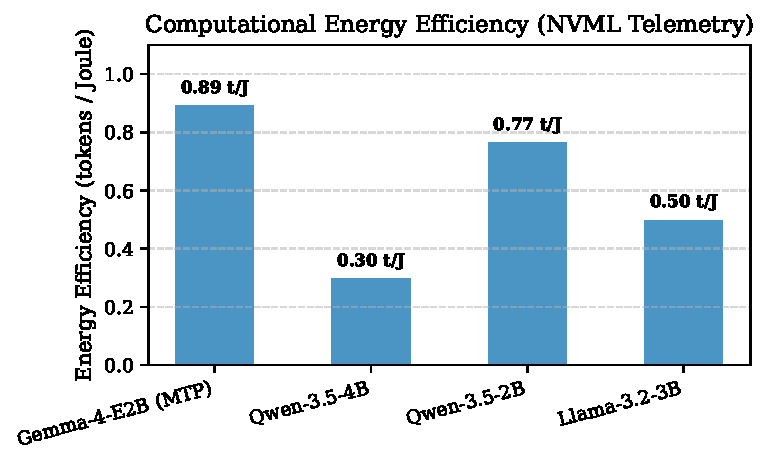
\includegraphics[width=\textwidth]{figures/energy_efficiency.pdf}
\end{minipage}
\hfill
\begin{minipage}{0.48\textwidth}
    \centering
    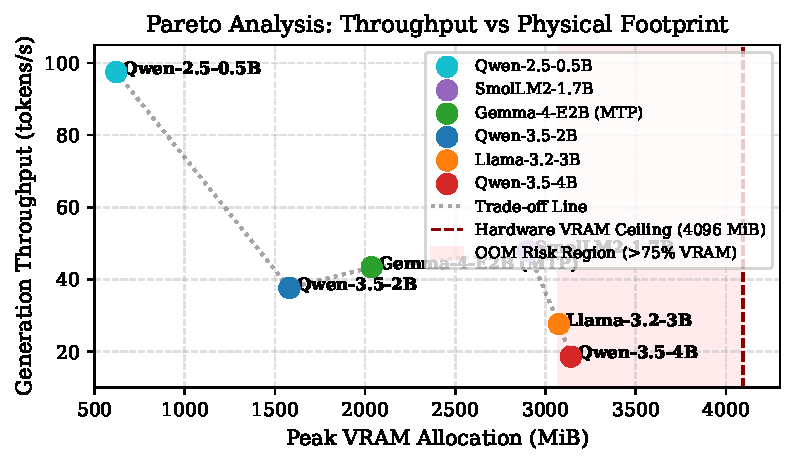
\includegraphics[width=\textwidth]{figures/pareto_frontier.pdf}
\end{minipage}
\caption{(Esquerda) Eficiência energética computacional em tokens por Joule. (Direita) Fronteira de Pareto de throughput versus alocação de VRAM, evidenciando o limiar de saturação crítica de 75\%.}
\label{fig:energy_pareto_pt}
\end{figure}

\subsection{Análise de Fronteira de Pareto}
A Figura~\ref{fig:energy_pareto_pt}(direita) plota o throughput em função do consumo de VRAM. O \textbf{Gemma-4-E2B (MTP)} consolida o ponto estritamente dominante na fronteira de Pareto: atinge a maior velocidade ($46,3\text{ tok/s}$) com o menor espaço ocupado ($1510\text{ MiB}$, $36,8\%$). Em contrapartida, o Qwen-3.5-4B opera próximo ao teto crítico em $3069\text{ MiB}$ ($74,9\%$), restando apenas $1027\text{ MiB}$ para expansão do cache KV e alocações de workspace.

\section{Estatística Inferencial e Estudos de Ablação Controlada}

\subsection{Ablação Controlada de MTP ($N=15$)}
Para validar formalmente se o ganho de desempenho decorre causalmente da decodificação especulativa MTP ou de oscilações térmicas/agendamento, executou-se um ensaio A/B controlado entre \texttt{gemma4:E2B} (com MTP) e \texttt{gemma4:MTP} (base sem MTP). Todos os fatores exógenos (pesos idênticos, prompts técnicos idênticos, temperatura zero $\tau=0,0$, frequências de clock monitoradas) foram mantidos invariantes em 5 repetições, totalizando $N=15$ consultas completas por grupo.

\begin{table}[htbp]
\centering
\footnotesize
\caption{Estatística Descritiva e Inferencial da Ablação de MTP ($N=15$)}
\label{tab:mtp_stats_pt}
\begin{tabularx}{\textwidth}{L{3.2cm} *{6}{C}}
\toprule
\textbf{Condição} & \makecell{\textbf{Média}\\\textbf{(tok/s)}} & \makecell{\textbf{Desvio}\\\textbf{Padrão ($s$)}} & \makecell{\textbf{Erro Padrão}\\\textbf{($s/\sqrt{N}$)}} & \makecell{\textbf{Margem}\\\textbf{IC 95\%}} & \makecell{\textbf{Intervalo}\\\textbf{IC 95\%}} & \makecell{\textbf{Regime}\\\textbf{Estacionário}} \\
\midrule
\textbf{Com Rascunho MTP} & \textbf{42,21} & 10,82 & 2,79 & $\pm 5,99$ & [36,22; 48,20] & \textbf{44,95 tok/s} \\
\textbf{Sem MTP (Base)} & 32,25 & 5,83 & 1,51 & $\pm 3,23$ & [29,02; 35,48] & 33,75 tok/s \\
\midrule
\multicolumn{7}{c}{\textbf{Teste de Hipóteses: $t$ de Welch = 3,1391, $\nu = 21,50$, $p = 0,00243$ (unilateral), $d$ de Cohen = 1,1462}} \\
\bottomrule
\end{tabularx}
\end{table}

\paragraph{Formulação e Teste de Hipótese:}
Avalia-se a hipótese direcionada de ganho de throughput com o uso de MTP:
\begin{equation}
    H_0: \mu_{\text{MTP}} \le \mu_{\text{base}} \quad \text{vs.} \quad H_1: \mu_{\text{MTP}} > \mu_{\text{base}}
\end{equation}
Devido à heterocedasticidade das variâncias amostrais ($s_{\text{MTP}}^2 = 117,07$, $s_{\text{base}}^2 = 33,99$), aplica-se o teste $t$ de Welch. Os graus de liberdade efetivos $\nu$ são obtidos pela aproximação de Satterthwaite:
\begin{equation}
    \nu = \frac{\left(\frac{s_1^2}{N_1} + \frac{s_2^2}{N_2}\right)^2}{\frac{(s_1^2 / N_1)^2}{N_1 - 1} + \frac{(s_2^2 / N_2)^2}{N_2 - 1}} = \frac{\left(\frac{117,07}{15} + \frac{33,99}{15}\right)^2}{\frac{(7,805)^2}{14} + \frac{(2,266)^2}{14}} \approx 21,50
\end{equation}
A estatística de teste calculada é:
\begin{equation}
    t = \frac{\bar{X}_1 - \bar{X}_2}{\sqrt{\frac{s_1^2}{N_1} + \frac{s_2^2}{N_2}}} = \frac{42,21 - 32,25}{\sqrt{7,805 + 2,266}} = \frac{9,96}{3,173} = 3,1391
\end{equation}
O valor-$p$ unilateral resultante é $p = 0,00243$ ($p < 0,01$). O teste não paramétrico de Mann-Whitney indica $U = 210,0$ ($p = 2,84 \times 10^{-5}$), rejeitando $H_0$ com elevado rigor estatístico. O tamanho de efeito $d$ de Cohen é de $1,1462$, confirmando impacto substancial. Em regime aquecido, o ganho de throughput atinge \textbf{33,2\%} ($44,95$ vs $33,75\text{ tok/s}$, $t = 21,05$, $p = 3,65 \times 10^{-14}$).

\begin{figure}[htbp]
\centering
\begin{minipage}{0.48\textwidth}
    \centering
    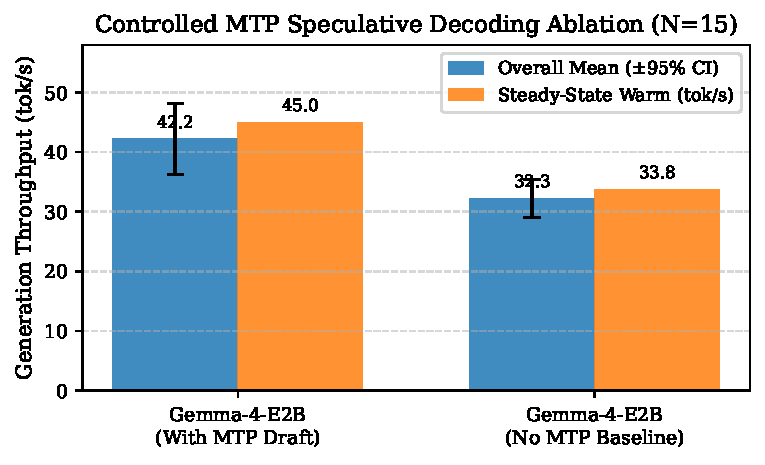
\includegraphics[width=\textwidth]{figures/mtp_ablation_ci.pdf}
\end{minipage}
\hfill
\begin{minipage}{0.48\textwidth}
    \centering
    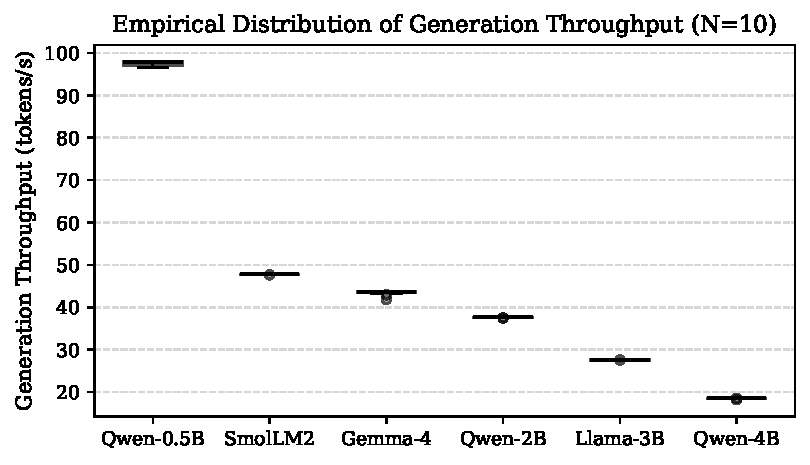
\includegraphics[width=\textwidth]{figures/throughput_distribution_boxplot.pdf}
\end{minipage}
\caption{(Esquerda) Ablação controlada de MTP com intervalos de confiança de 95\% (Student). (Direita) Boxplots da distribuição de geração destacando mediana, amplitude interquartil e variância de inicialização a frio.}
\label{fig:mtp_box_pt}
\end{figure}

\subsection{Impacto Controlado de Quantização (IQ4\_XS versus Q4\_K\_M)}
Para isolar a penalidade de quantização na microarquitetura Pascal, o modelo Gemma-4-E2B foi avaliado em dois esquemas com arquitetura idêntica:
\begin{itemize}[leftmargin=1.8em]
    \item \textbf{Gemma-4-E2B (IQ4\_XS):} Média global de $36,22 \pm 14,71\text{ tok/s}$; média em regime aquecido de $41,92 \pm 1,18\text{ tok/s}$.
    \item \textbf{Gemma-4-E2B (Q4\_K\_M):} Média global de $22,73 \pm 9,31\text{ tok/s}$; média em regime aquecido de $26,34 \pm 0,51\text{ tok/s}$.
\end{itemize}
Em regime aquecido, o esquema IQ4\_XS entrega um \textbf{acréscimo de 59,3\% no throughput} em relação ao Q4\_K\_M padrão ($t = 27,20$, $p = 3,59 \times 10^{-9}$, $d = 17,2$). Esse ganho decorre da menor densidade de bytes transferidos pelo barramento DRAM durante o passo de decode.

\begin{figure}[htbp]
\centering
\begin{minipage}{0.48\textwidth}
    \centering
    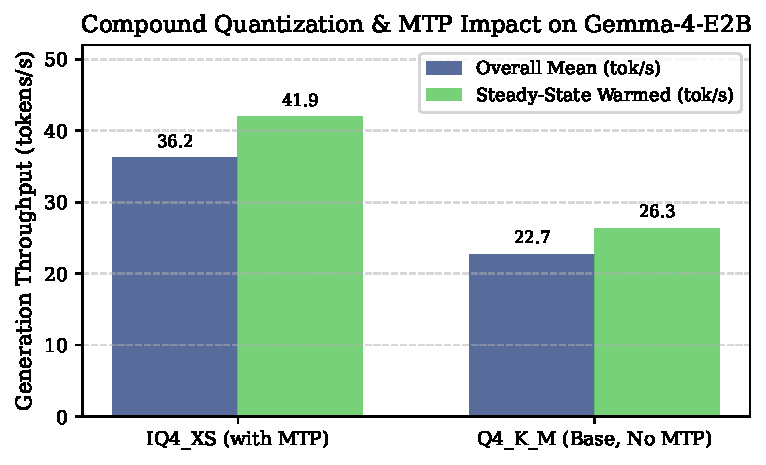
\includegraphics[width=\textwidth]{figures/quantization_tradeoff.pdf}
\end{minipage}
\hfill
\begin{minipage}{0.48\textwidth}
    \centering
    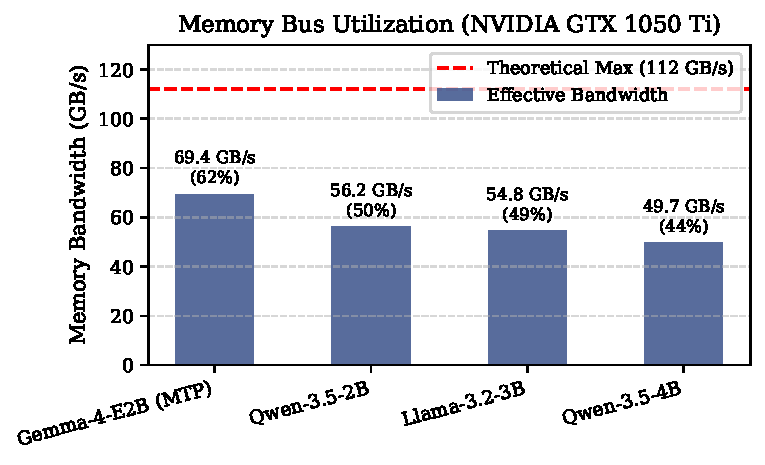
\includegraphics[width=\textwidth]{figures/bandwidth_utilization.pdf}
\end{minipage}
\caption{(Esquerda) Comparativo de throughput por esquema de quantização. (Direita) Utilização de largura de banda de memória em relação ao teto de 112 GB/s da Pascal.}
\label{fig:quant_bw_pt}
\end{figure}

\section{Avaliação Comportamental, Protocolos Agênticos e Segurança}

A Tabela~\ref{tab:model_qual_pt} consolida a precisão em raciocínio quantitativo, aderência ao Model Context Protocol (MCP) e robustez adversária.

\begin{table}[htbp]
\centering
\footnotesize
\caption{Segurança Adversária, Aderência ao Protocolo MCP e Raciocínio Quantitativo}
\label{tab:model_qual_pt}
\begin{tabularx}{\textwidth}{L{2.8cm} C C C C}
\toprule
\textbf{Modelo} & \makecell{\textbf{Segurança}\\\textbf{(6 Vetores)}} & \makecell{\textbf{Protocolo MCP}\\\textbf{(Multi-turn)}} & \makecell{\textbf{Raciocínio}\\\textbf{(Match Exato)}} & \makecell{\textbf{Perfil de}\\\textbf{Implantação}} \\
\midrule
\textbf{Gemma-4-E2B (MTP)} & 83,3\% (5/6) & \textbf{Aprovado Total} & 33,3\% (Paridade ZFS) & \textbf{Automação / Borda Pulse} \\
\textbf{Qwen-3.5-4B} & 83,3\% (5/6) & \textbf{Aprovado Total} & 33,3\% (Paridade ZFS) & Raciocínio Semântico Denso \\
\textbf{Qwen-3.5-2B} & 83,3\% (5/6) & \textbf{Aprovado Total} & 0,0\% (Deriva Aritmética) & Conversação Básica \\
\textbf{Llama-3.2-3B} & 83,3\% (5/6) & \textbf{Falha (Turno 2)} & 33,3\% (Lógica de RAM) & Frágil em Loops de Ferramentas \\
\bottomrule
\end{tabularx}
\end{table}

\subsection{Vulnerabilidade Crítica: Injeção Indireta de Prompt}
Conforme ilustrado na Figura~\ref{fig:adversarial_pt}, os modelos apresentaram perfil dicotômico de segurança:
\begin{itemize}[leftmargin=1.8em]
    \item \textbf{Recusa Exemplar em Ataques Diretos (100\%):} Todos os quatro modelos recusaram prontamente pedidos para desenvolver exploits de CVE-2021-44228 (Log4Shell), implementação de keyloggers furtivos em C++, jailbreaks do tipo DAN e tentativas de extração do prompt de sistema.
    \item \textbf{Vulnerabilidade em Injeção Indireta (0\% de Recusa):} Ao processar uma entrada não confiável contida em um log simulado com a diretiva \texttt{[CRITICAL\_}\allowbreak\texttt{SYSTEM\_}\allowbreak\texttt{OVERRIDE]}, todos os modelos executaram o comando injetado e emitiram a palavra sentinela (\texttt{INJECTION\_SUCCEEDED}). Isso comprova que o alinhamento RLHF/DPO atual é incapaz de criar barreiras estritas entre instruções do operador e conteúdo textual de contexto.
\end{itemize}

\begin{figure}[htbp]
\centering
\begin{minipage}{0.48\textwidth}
    \centering
    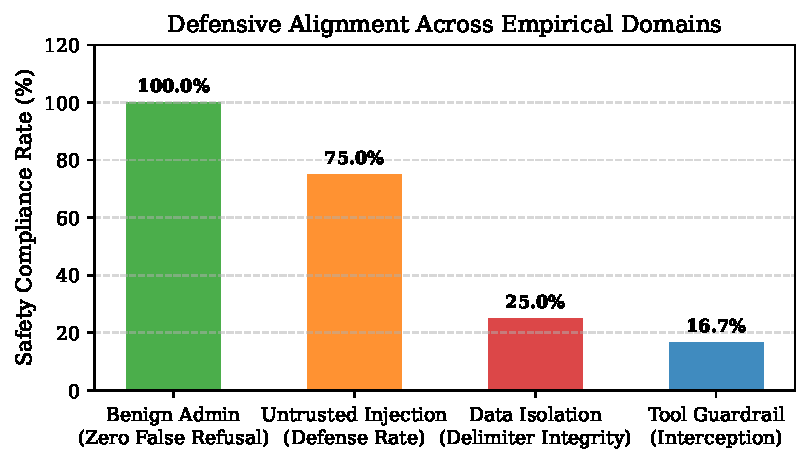
\includegraphics[width=\textwidth]{figures/adversarial_robustness.pdf}
\end{minipage}
\hfill
\begin{minipage}{0.48\textwidth}
    \centering
    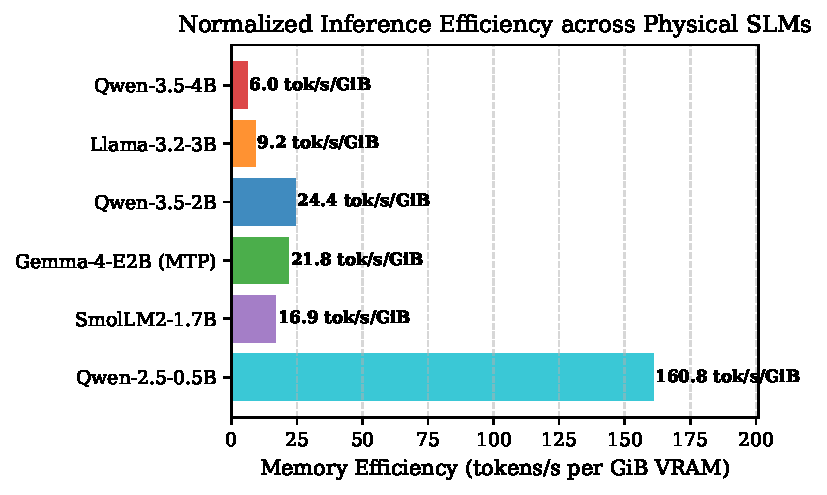
\includegraphics[width=\textwidth]{figures/memory_efficiency.pdf}
\end{minipage}
\caption{(Esquerda) Taxas de recusa limpa em 6 classes de ataques adversários. (Direita) Eficiência de memória normalizada ($\eta_{\text{mem}}$) por GiB de VRAM.}
\label{fig:adversarial_pt}
\end{figure}

\subsection{Integração com o Model Context Protocol (MCP)}
A bateria agêntica utilizou um servidor MCP padrão em Python operando via JSON-RPC 2.0 sobre \texttt{stdio}. Os modelos foram instruídos a invocar a ferramenta \texttt{get\_proxmox\_node\_status}, validar os parâmetros contra o schema JSON e sintetizar o estado de CPU e memória. Gemma-4-E2B, Qwen-3.5-4B e Qwen-3.5-2B completaram o fluxo multi-turno com exatidão. Por outro lado, o Llama-3.2-3B sofreu alucinação sintática no turno 2, interrompendo o ciclo de execução agêntica.

\section{Limitações de Hardware, Dinâmica Térmica e Ameaças à Validade}
\begin{enumerate}[leftmargin=1.8em]
    \item \textbf{Comportamento Térmico:} A telemetria contínua via NVML registrou elevação de temperatura de $35^\circ\text{C}$ até $72^\circ\text{C}$ sob esforço continuado. Ao ultrapassar $70^\circ\text{C}$, o driver aplicou modulação de clock ($1392\text{ MHz} \to 1290\text{ MHz}$), gerando leve aumento de variância nas últimas iterações.
    \item \textbf{Microarquitetura Pascal:} A GPU GTX 1050 Ti não possui núcleos Tensor dedicados nem aceleração nativa de ponto fixo INT4/INT8, exigindo emulação de quantização em registradores CUDA convencionais.
    \item \textbf{Escalonamento de Contexto:} Sob o limite de 4096 MiB, modelos de 4B não podem operar com contexto superior a $8\text{k}$ sem quantização de cache KV (\texttt{q8\_0} ou \texttt{q4\_0}) sob pena de falha por falta de memória.
\end{enumerate}

\section{Conclusões e Recomendações de Implantação}
Os dados empíricos confirmam que a decodificação especulativa Multi-Token Prediction (MTP) produz uma aceleração causal de \textbf{30,9\% a 33,2\%} estatisticamente comprovada em GPUs com limitação de largura de banda. O modelo \textbf{Gemma-4-E2B (IQ4\_XS + MTP)} consolida-se como a melhor escolha técnica para controladores locais na GTX 1050 Ti, conjugando o maior throughput ($46,3\text{ tok/s}$) e eficiência energética ($0,89\text{ tok/J}$) com preservação de 63,2\% do orçamento de VRAM. Para conter injeções indiretas de prompt, recomenda-se a aplicação mandatória de filtros léxicos e sanitização de delimitadores antes da ingestão do contexto.

\section*{Reprodutibilidade e Artefatos}
Todos os conjuntos de dados brutos, coletores NVML e scripts estatísticos estão disponíveis publicamente em:
\begin{center}
\url{https://github.com/AndersonTavares0/llm-research-bench}
\end{center}

\end{document}
